\documentclass{beamer}
\usepackage{graphicx} 
\usepackage{tikz}
\usepackage{color}
\newcommand{\btVFill}{\vskip0pt plus 1filll}
\usepackage[export]{adjustbox} 
\usetheme{Szeged}
\usecolortheme{wolverine}
\usepackage{wrapfig}
%Information to be included in the title page:
\title{Improving Laser Guide Stars through Magnetic Resonant Pulsing}
\author{Adam Newton Wright}
\institute{Willamette University}
 
\begin{document}
 {
	\usebackgroundtemplate{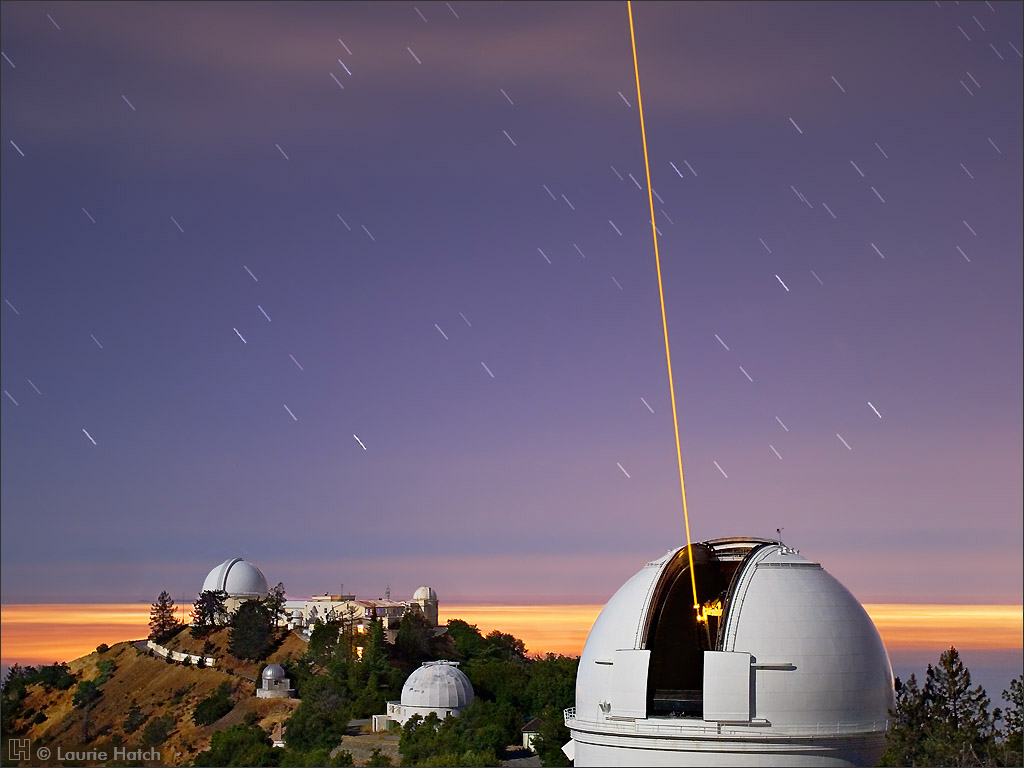
\includegraphics[width=\paperwidth,height=\paperheight]{Images/lgs_livermore.jpg}}
	%TITLE FRAME
	\begin{frame}
	  \color{white}
	  \titlepage
	  \bigskip
	  \btVFill
	  {\tiny Bishop, Brianna, ``Bringing New Life to Laser Guide Star,''Lawrence Livermore National Laboratory, June 2014}\\

	\end{frame}
  }


  %FIRST FRAME: OVERVIEW okay
\begin{frame}
  \frametitle{Overview}
  \begin{itemize}
	\item Laser Guide Stars
	  \begin{itemize}
		\item{What are Laser Guide Stars used for?}
		\item{What is a Laser Guide Star?}
	  \end{itemize}
	\item Optical Pumping 
	  \begin{itemize}
		\item How it works
		\item{Geomagnetic Field Complications}
		\item{Larmor Precession}
		\item{How MRP can be a solution}
	  \end{itemize}
	\item Our Experiment
	  \begin{itemize}
		\item{Hypothesis}
		\item Dye Lasers
		\item{Lasing Frequency}
		\item{Sodium Housing and Magnetic Field}
		\item{Measurements and Comparison}
	  \end{itemize}
  \end{itemize}
\end{frame} 




%%Third Frame: Laser Guide Stars: What are they used for?
\begin{frame}
  \frametitle{Laser Guide Stars (LGS)}
  \framesubtitle{What are LGSs used for?}
  \begin{itemize}
	\item Astronomers need clearer images; limited by atmosphere\\
	\item Employ adaptive optics (AO) systems$^1$
	\item AO corrects distortions that occur as light enters atmosphere \\
	\item Need something bright the sky to measure these distortions
	  \begin{minipage}{.5\textwidth}
	  \begin{itemize}
		\item Use a star, but not always a bright star in all parts of the sky
		\item Create an artificial star, i.e. LGS
	  \end{itemize}
	\end{minipage}
  \end{itemize}
  \hfill
  \begin{minipage}{.4\textwidth}
	\begin{center}
	  \vspace{-2cm}
	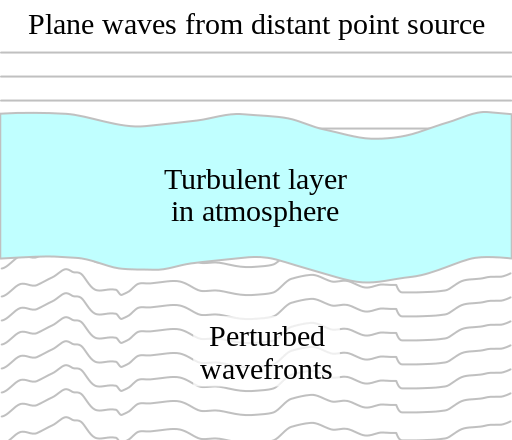
\includegraphics[width = 3cm, height = 3cm]{Images/adaptiveoptics1.png}
  \end{center}
  \end{minipage}
	  \bigskip
	  \btVFill
	  {\tiny $^1$Wizinowich, "The WM Keck Observatory laser guide star adaptive optics system: overview." Publications of the Astronomical Society of the Pacific 118, no. 840 (2006): 297.
}\\
\end{frame}


%% Second Frame: Laser Guide Stars: What are they?
\begin{frame}
  \frametitle{Laser Guide Stars (LGS)}
  \framesubtitle{What are they?}
  \begin{minipage}{.6\textwidth}
  \begin{itemize}
	\item Artificial star created by laser light\\
	\item Two Types:\\
	  \begin{itemize}
		\item Sodium beacon
		\item Rayleigh Scattering
	  \end{itemize}
	\item Sodium LGS excites sodium in the mesosphere$^2$
	\item Rayleigh scattering LGS scatters laser light in the lower atmosphere$^2$
	  
  \end{itemize}
\end{minipage}
\begin{minipage}{.35\textwidth}
  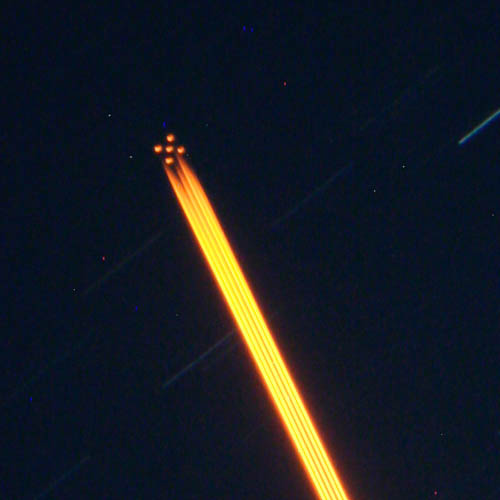
\includegraphics[width = 4cm, height = 5.5cm]{Images/lgs_insky.jpg}
  \end{minipage}
	  \bigskip
	  \btVFill
	  {\tiny  $^2$``Laser Guide Star,'' RP Photonics, 2016}\\
	  {\tiny ``Laser-Guide Star HD Videos and Imagesi,`` Gemini Observatory/AURA, gemini.edu, 2013 }\\
\end{frame}





%% Fourth Frame: Laser guide star: How to create a LGS
\begin{frame}
  \frametitle{Laser Guide Stars (LGS)}
  \framesubtitle{Sodium LGS}
  Sodium Laser Guide Star System\\
  \begin{itemize}
	\item Mesospheric sodium layer: 10 km thick and 90 km in altitude\\
	  \begin{itemize}
		\item Created by the ablation of meteors
	  \end{itemize}
  \end{itemize}
  \begin{minipage}{.45\textwidth}
  \begin{itemize}
	\item Wavenlength $\lambda=$ 589.593 nm\\
	\item Intensity$^3$ $I \approx 10 Wm^{-2}$
	\item Circularly polarized light $\sigma ^+$
  \end{itemize}
\end{minipage}
\begin{minipage}{.35\textwidth}
  \begin{tikzpicture}
	\node at (0,0) {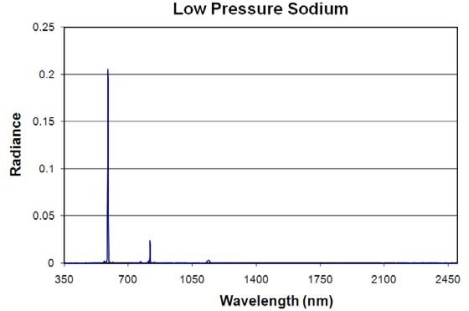
\includegraphics[width = 6cm, height = 3.5cm]{Images/sodium_emission.png}};
\end{tikzpicture}
\end{minipage}
	  %\bigskip
	 %\btVFill
	 \\{\tiny $^3$Schock, M., et al. "Performance analysis of polychromatic laser guide stars used for wavefront tilt sensing." Monthly Notices of the Royal Astronomical Society 337.3 (2002)}\\
 
	  {\tiny Elvidge CD et al, ``Spectral identification of lighting type and character.`` Earth Observation Group}\\
\end{frame}





%% Ninth Frame: Larmor Precession: optical pumping 
\begin{frame}
  \frametitle{Optical Pumping}
  \framesubtitle{How it works}
  \begin{itemize}
	\item Optical pumping uses circularly polarized light to exite atoms
	  \begin{columns}
		\column{.5\textwidth}
	  \begin{itemize}
		\item Atoms that scatter circularly polarized light move to different angular momentum state
		\item This angular momentum state has increases chance of backscattering photons (cycling)$^4$\\
	  \end{itemize}
  \column{.5\textwidth}
  \begin{tikzpicture}
	\node at (0,0) {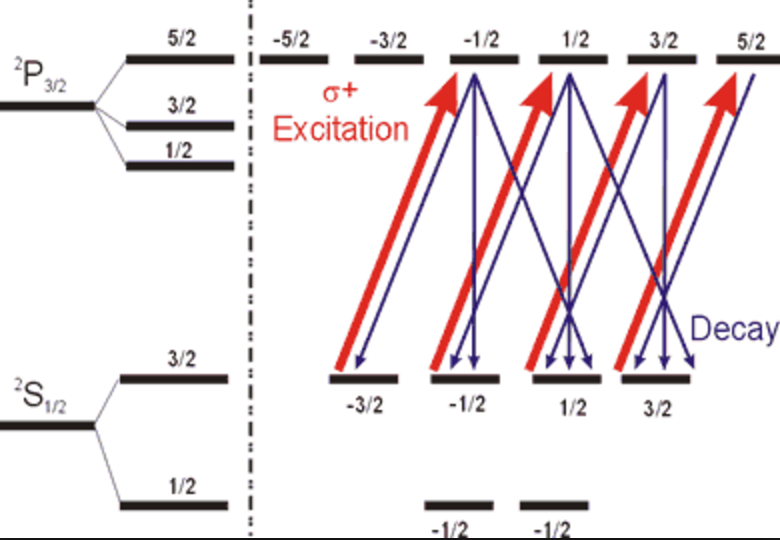
\includegraphics[width = 4cm, height = 3cm,left]{Images/opticalpumping.png}};
	\node at (-2.3,0) {\footnotesize $\Delta m = \pm 1,0$};
	\onslide<2>{ \draw [blue, line width = 1.6pt,rotate = -15 ] (.7,.4) ellipse (.5cm and 1.5cm);
	  \node at (2,0) [blue] {Cycling};}
  \end{tikzpicture}
\end{columns}
  \end{itemize}
\\{\tiny $^4$Kane, "Pulsed laser architecture for enhancing backscatter from sodium." SPIE Astronomical Telescopes+ Instrumentation. International Society for Optics and Photonics, 2014.}\\
{\tiny ``Spin polarization by optical pumping,'' Colinear Laser Spectroscopy, 2013}
 
\end{frame}


%%9.5 Frame: Larmor Precession: a complication

\begin{frame}
  \frametitle{Optical Pumping}
  \framesubtitle{Geomagnetic Field Complications}
  \begin{itemize}
	\item Optical pumping most efficient when $\vec B$ $||$   laser beam$^5$
	\item When $\vec B \perp$  laser beam, benefits of optical pumping eliminated
	  \begin{minipage}{.5\textwidth}
	\item Most telescopes have are close to equator
	  \begin{itemize}
		\item Large $\perp \vec B$ component
	  \end{itemize}
	\item Want to find to way to keep optical pumping benefits at all magnetic orientations
	\end{minipage}
  \end{itemize}
\hfill
\begin{minipage}{.35\textwidth}
  \begin{center}
	\vspace{-3cm}
	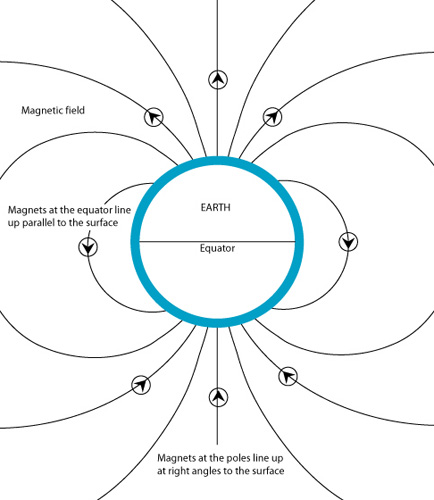
\includegraphics[width = 3cm, height = 3cm]{Images/magneticfield.jpg}
\end{center}
\end{minipage}
  \bigskip
 \\ {\tiny $^5$Rampy, Rachel, Donald Gavel, Simon M. Rochester, and Ronald Holzlöhner. "Toward optimization of pulsed sodium laser guide stars." JOSA B 32, no. 12 (2015): 2425-2434.}


\end{frame}



%% Eighth Frame: Larmor Precession: In Magnetic Fields

\begin{frame}
  \frametitle{Optical Pumping}
  \framesubtitle{Larmor Precession}
  \begin{itemize}
	\item Larmor precession: precession of any magnetic moment in any magnetic field\\
	\item Sodium has a magnetic moment and thus precesses\\
  \end{itemize}
  %\vspace{-.4cm}
	  \begin{minipage}{0.4\textwidth}
		\vspace{-3cm}
	  \begin{center}
		 $\vec \tau = \vec \mu \times \vec B $\\
	   $\omega = -\gamma B$\\
	   $ \gamma = \frac{eg}{2m}$
	\end{center}
  \end{minipage}
  \hfill
  \begin{minipage}[b]{0.4\textwidth}
  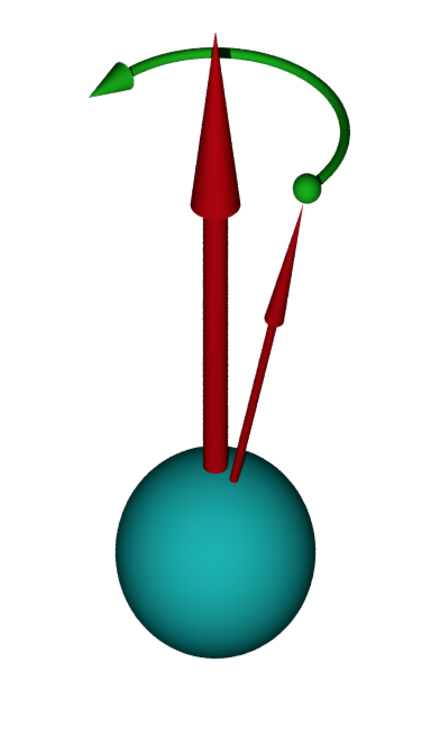
\includegraphics[width = 2cm, height = 3cm]{Images/larmorprecession.png}
  \end{minipage}
	\\\scriptsize{where $\tau$ is the torque exerted, $\mu$ is the magnetic dipole moment, $B$ is the external magnetic field, $\omega$ is the angular frequency, and $\gamma$ is the gyromagnetic ratio with $e$ being the electric charge, $g$ being the \textit{g-factor}, and $m$ being the mass of the object.}
\end{frame}





%% Tenth Frame: Larmor Precession: A solution
\begin{frame}
  \frametitle{Optical Pumping}
  \framesubtitle{A Solution}
  \begin{itemize}
	\item Magnetic Resonant Pulsing (MRP):$^6$\\
	  \begin{itemize}
		\item Laser is pulsed at a frequency corresponding to atom's Larmor frequency\\
		\item Light only interacts with atom at one point in precession cycle\\
		\item Atom can properly redistribute its angular momentum\\
	  \end{itemize}
	\item MRP has only been simulated, not experimented\\
  \end{itemize}
  \bigskip
{\tiny $^6$Kane, "Pulsed laser architecture for enhancing backscatter from sodium." SPIE Astronomical Telescopes+ Instrumentation. International Society for Optics and Photonics, 2014.}\\
\end{frame}







%% Eleventh frame: Our experiment: Hypothesis
\begin{frame}
  \frametitle{Our Experiment}
  \framesubtitle{Hypothesis}
  \begin{itemize}
	\item Hypothesis: Magnetic resonant pulsing of sodium results in greater emission at all angles between beam and magnetic field than excition without MRP.\\
	\item Experimentally test the computer simulation of Kane et al.
  \end{itemize}
  \begin{center}
	\begin{tikzpicture}
	  \node at (0,0) {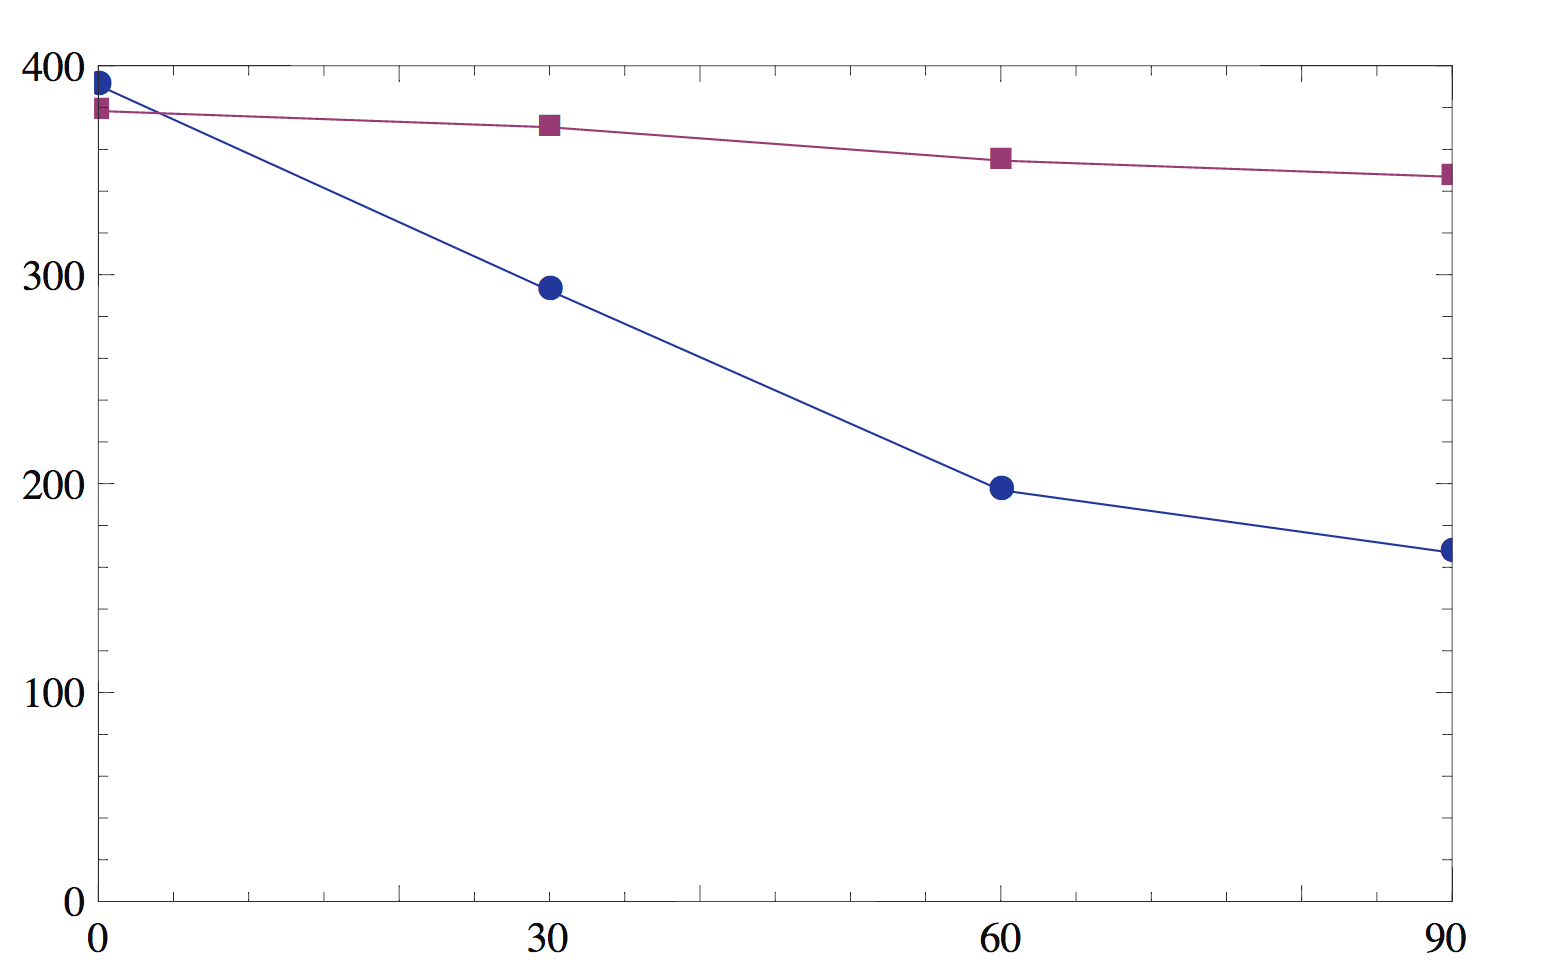
\includegraphics[width = 7cm, height = 3cm]{Images/hilmangraph1.png}};
	  \node at (-4,0) [rotate = 90] {Emission $Wm^{-2}$};
	  \node at (0,-1.8) {Angle between $\vec B$ and laser beam};
  \end{tikzpicture}
\end{center}
{\tiny Kane, "Pulsed laser architecture for enhancing backscatter from sodium." SPIE Astronomical Telescopes+ Instrumentation. International Society for Optics and Photonics, 2014.}\\
\end{frame}

%% 11.5 frame: Our experiment: Outline
\begin{frame}
  \frametitle{Our Experiment}
  \framesubtitle{Outline}
  \begin{itemize}
	\item Create MRP dye laser
	\item Sodium confinement and magnetic field
	\item Spectroscopy measurements
  \end{itemize}
\end{frame}

	%Sixth FRAME: DYE LASERS: SYSTEM OVERVIEW
\begin{frame}
  \frametitle{Our Experiment}
  \framesubtitle{Dye Lasers}
  \begin{itemize}
	\item Excellent tunability over close to one hundred nanometers
	\item Lasing medium: organic fluid dye solution\\ 
	\item Pumping: Laser light excites dye solution\\
	\item Cavity: Two mirrors and a diffraction grating\\
	\item Diffraction grating allows wavelength to be selected\\
  \end{itemize}
  \begin{tikzpicture}
	\node at (0,0) {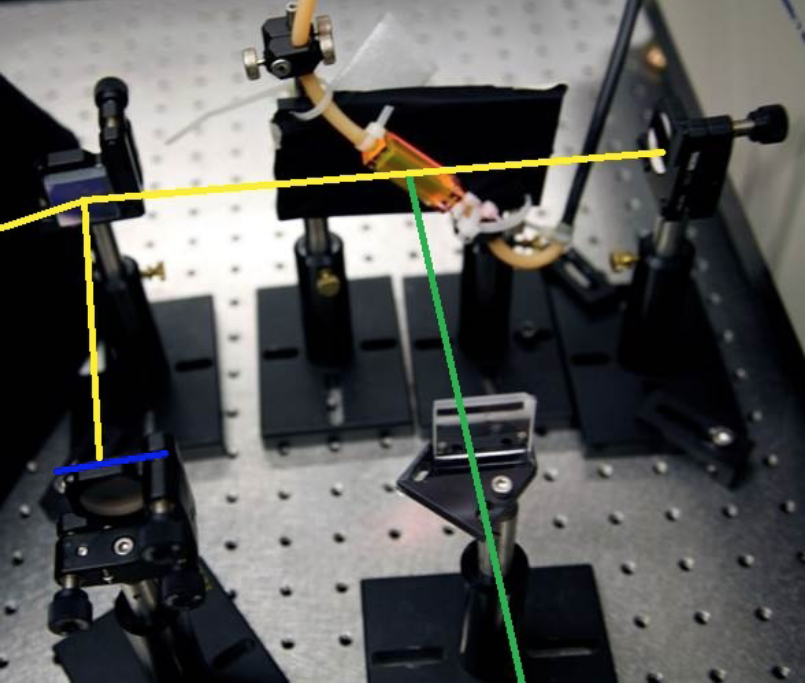
\includegraphics[width = 6cm, height = 3.5cm,center]{Images/dyelaser_hayley.png}};
	\node at (.8,1.5) [white] {Dye Cell};
	%\draw [white, line width = 1.6pt] (0,1.3) rectangle (1.6, 1.8);
	\node at (2,-1.5) [green, line width = 1.6pt]  {Pump Beam};
	\node at (-2,1.5) [white, line width = 1.6pt]  {Grating};
\end{tikzpicture}
  \bigskip
  { \tiny``Construction of a Dye Laser for Use in Detecting Ultracold RbCa,'' Hayley Whitson, Willamette University, 2012`}

\end{frame}







%% Seventh Frame: Dye Lasers: Our dye laser
\begin{frame}
  \frametitle{Our Experiment}
  \framesubtitle{Our Dye Laser}
  \begin{itemize}
	\item Moya cavity creates lasing and minimizes spontaneous emission\\
	\item Two amplification cells intensify output beam\\
	\item Pump with kilohertz, picosecond pump beam
  \end{itemize}
  \begin{columns}
	\column{.5\textwidth}
\center	Dye laser schematic
	\begin{tikzpicture}
	  \node at (0,0) {\includegraphics[scale =.25,left]{Images/ND6K.png}};
	  \node at (0,0) [blue] {Cell};
	  \draw [blue,line width = 1.6pt] (.4,-.4) circle [radius = .3];
  \end{tikzpicture}
  \column{.5\textwidth}
  \center Moya cavity
  \begin{tikzpicture}
	\node at (0,0) {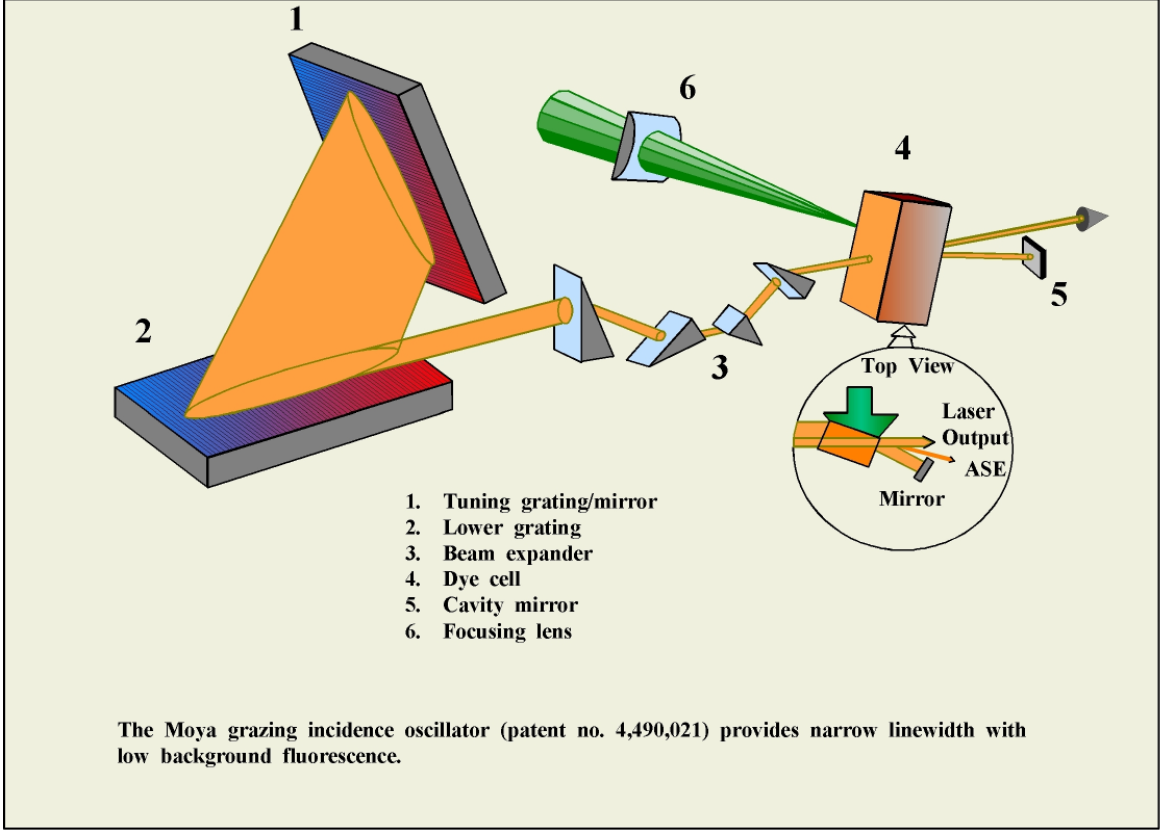
\includegraphics[height = 3cm, width = 4cm]{Images/moya_cavity.png}};
\end{tikzpicture}
  \end{columns}
 \\ {\tiny `` ND6K User Manual,'' Contiuum Lasers, 1994}
\end{frame}


\begin{frame}
  \frametitle{Our Experiment}
  \framesubtitle{Sodium Housing and Magnetic Field}
  \begin{itemize}
	\item Sodium housed in a reference cell
	\item Magnetic coils on either side of reference frame
	  \begin{itemize}
		\item Rotate to change angle between laser and $\vec B$
	  \end{itemize}
	\item Dye laser shone into reference cell and collected by photodiode
  \end{itemize}
  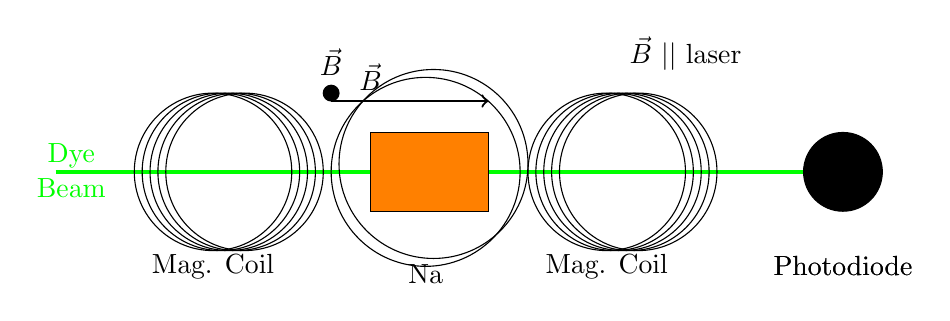
\begin{tikzpicture}
	\draw [green, ultra thick] (0,1) -- (10,1);
	\onslide<1> {\draw (2,1) circle [radius = 1];
	\draw (2.1,1) circle [radius = 1];
	\draw (2.2,1) circle [radius = 1];
	\node at (8,2.5) {$\vec B$ $||$ laser};
	\draw (7,1) circle [radius = 1];
	\draw (7.1,1) circle [radius = 1];
	\draw (7.2,1) circle [radius = 1];
	\draw (7.3,1) circle [radius = 1];
  \draw (7.4,1) circle [radius = 1];
	\draw (2.3,1) circle [radius = 1];
	\draw [thick, ->] (3.5,1.9) -- (5.5,1.9);
	\node at (4,2.2) {$\vec B$};
	\draw (2.4,1) circle [radius = 1];}
	\draw [fill = orange] (4,.5) rectangle (5.5,1.5);
	\draw [fill = black] (10,1) circle [radius=.5];
	\node at (4.7,-.3) {Na};
	\node at (2,-.2) {Mag. Coil};
	\node at (7,-.2) {Mag. Coil};
	\node at (10,-.2) {Photodiode};
	\node [green] at (.2,1.2) {Dye};
	\node [green] at (.2,.8) {Beam};
	\onslide<2>{ \draw (4.7,1) circle [radius = 1.2, ultra thick];
	\node at (10,-.2) {Photodiode};
	\node at (3.5,2.4) {$\vec B$};
	\draw [fill = black] (3.5,2) circle [radius = .1];
	\draw (4.8,1.1) circle [radius = 1.2, ultra thick];}
  \end{tikzpicture}
\end{frame}

\begin{frame}
  \frametitle{Our Experiment}
  \framesubtitle{Spectroscopy Measurements}
  \begin{itemize}
	\item Take absorption spectroscopy measurements
	  \begin{itemize}
		\item $\vec B$ along one direction
		\item Measure absorption as $\lambda$ changes
		\item Change direction of $\vec B$ and repeat
	  \end{itemize}
  \end{itemize}
  \begin{center}
		\begin{tikzpicture}
		  \node at (0,0) {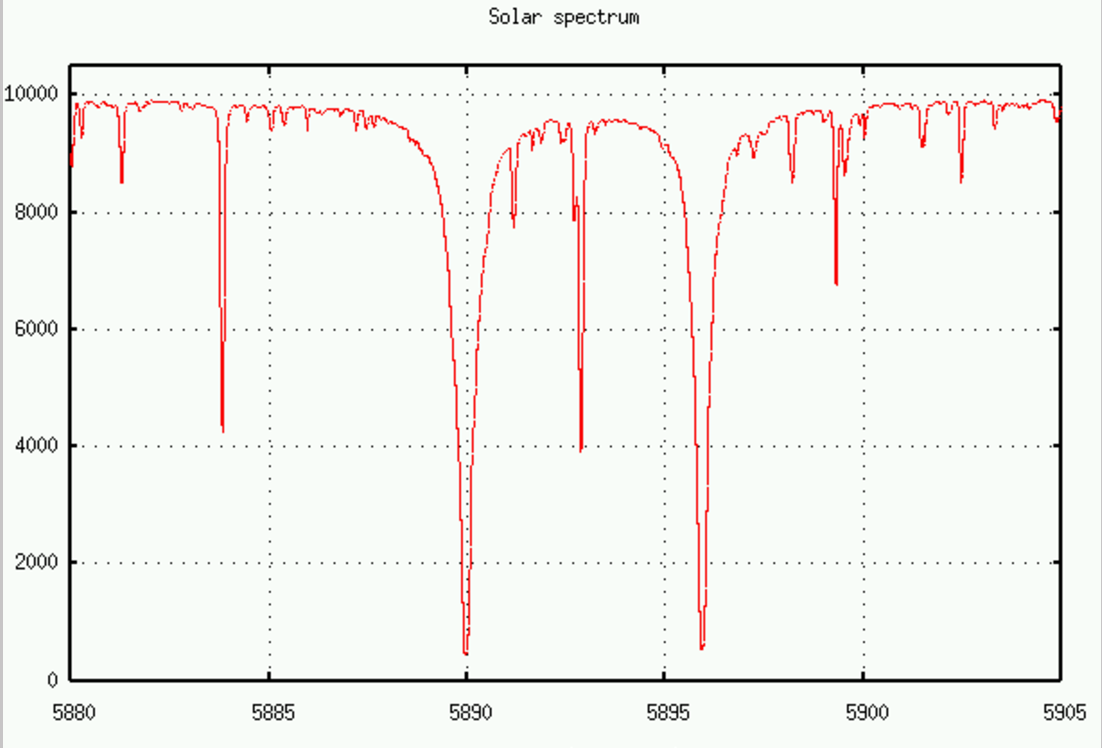
\includegraphics[width = 8cm, height = 3cm]{Images/absorbtionspectroscopy2.png}};
		  \node at (-4.5,0) [rotate = 90] {\footnotesize Intensity};
		  \node at (0,-1.7) {\footnotesize Wavelength (nm)};
		  \onslide<2> {\draw [blue, line width = 1.6pt](.7,-1.3) rectangle (1.8,1.3);
		  \node at (1.8,1.9) [blue] {589.6 nm};}
	\end{tikzpicture}
  \end{center}
  \\{\tiny Michael Richmond, Rochester Institute of Technology, \textit{spiff.rit.edu/classes/phys440/lectures/curve}}
\end{frame}

\begin{frame}
  \frametitle{Our Experiment}
  \framesubtitle{Data Analysis}
  \begin{itemize}
	\item Data will be taken with the laser pulsed at the Larmor frequency, and at a frequency not equal to the Larmor frequency
	\item These data will be compared by looking at the highest absorption of sodium
  \end{itemize}
\end{frame}


\begin{frame}
  \frametitle{Conclusion}
  \begin{itemize}
	\item Laser guide stars, and what they are used for
	\item Optical pumping and the geomagnetic field
	\item How MRP can solve this problem
	\item Our experiment to test MRP
  \end{itemize}
\end{frame}

\begin{frame}
  \frametitle{Thank you all for wathcing my presentation!}
  Also, thank you
  \begin{itemize}
	\item Michaela Kleinert, for your endless help
	\item The Physics Department, for always being amazing
	\item Donald Swen, for all the hours we have struggled in lab together
  \end{itemize}
\end{frame}

{
\usebackgroundtemplate{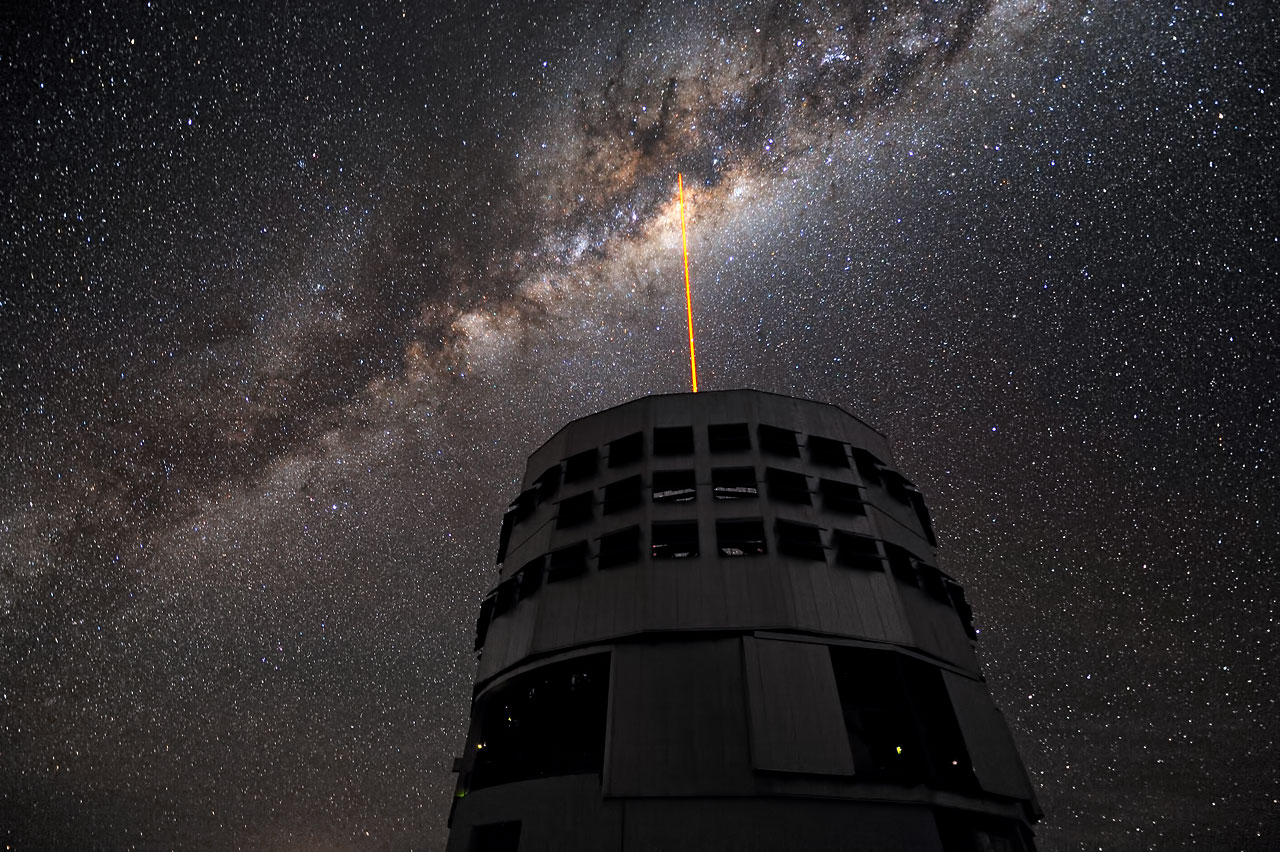
\includegraphics[width=\paperwidth,height=\paperheight]{Images/ending_lgs.jpg}}
\begin{frame}
\frametitle{Questions?}
\bigskip
\bigskip
\vspace{6cm}
\bvTFill
\color{white}
\tiny{``Staight to the Milky Way's Heart,'' Scientific Computing, 2011}
\end{frame}
}
\end{document}

%% References
%% Background Image
%% Bishop, Brianna, ``Bringing New Life to Laser Guide Star,''Lawrence Livermore National Laboratory, June 2014

%% 4 LGS in sky
%%Gemini Observatory/AURA, gemini.edu, `` laser-Guide Star HD Videos and Images``


%% sodium emission graph
%% Elvidge CD et al, `` spectral identification of lighting type and character.``  Earth Observation Group

%% Dye laser: Hayley whitson
%% Whitson, Hayley, Senior Thesis, Willamette University, 2012

%% Moya Cavity 
%% Continuum ND6k Manual


%% Larmor precession
%% wikipedia larmor precession

%%Optical pumping
%% Spin polarization byoptical pumping, Colinear laser spectroscopy
